\documentclass{article}

\usepackage[english]{babel}

\usepackage{float}
\usepackage{amsmath}
\usepackage{graphicx}
\usepackage{hyperref}
\usepackage[caption = false]{subfig}
\usepackage[colorlinks=true, allcolors=blue]{hyperref}
\hypersetup{
    colorlinks=true,
    linkcolor=blue,
    filecolor=magenta,      
    urlcolor=cyan,
    }
\title{Street Fighter with Relational Inductive Biases} 
\author{Ashutosh Tiwari (@ashutiwa)}

\begin{document}
\maketitle

\section{Problem}

Street Fighter is one of the most explored games for reinforcement learning research. It is available as one of the environments in Gym Retro. However in almost all approaches the state is represented by scene frames. In this project I am trying to apply Relational Inductive Biases to this problem. 
This project takes a lot of ideas from \href{https://openreview.net/pdf?id=HkxaFoC9KQ}{this} paper. In this case we are trying to use relationships between entities in a scene to figure out the best behaviour of our agent. These relationships are not encoded but are learned by the network itself.

\section{Algorithm}

I will start with A2C where $\pi$ (actor) which is the output of the network, are logits over set of actions, at a state $s$. From these logits an action is sampled. Baseline value is the critic, $B$ which is the estimate of the state-value function.

This is very similar to the paper I referenced above. Few changes will be that the state will include current health and difference in positional embeddings (not sure) as well.

$B$ is used to compute temporal difference error. Then this error is used to optimize $\pi$ and optimize $B$.

\section{Architecture}
Architecture is more or less similar to above paper. Even if there are little changes, this overall architecture is copied from that paper.

\begin{figure}[H]
\centering
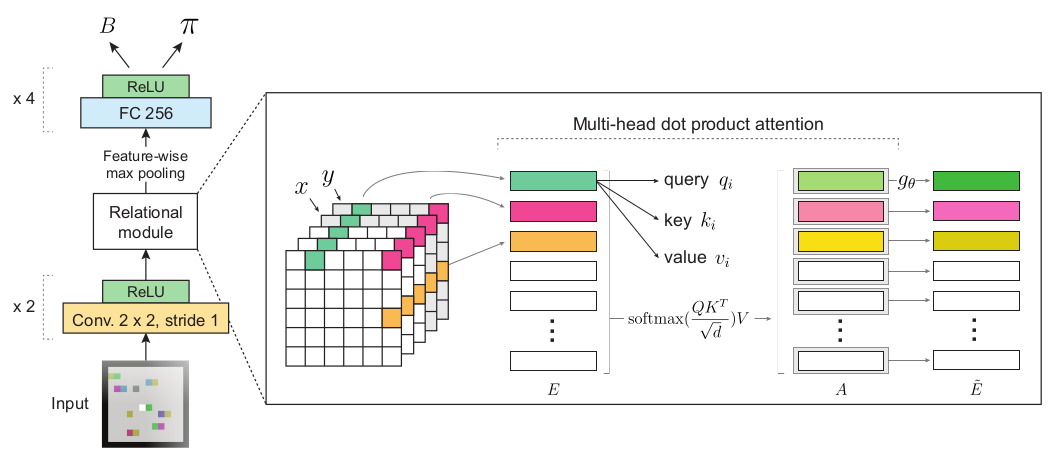
\includegraphics[width=3.8in]{Screenshot from 2022-03-30 22-16-29.png}
\caption{Architecture}
\end{figure}


\section{Experiments}
\begin{itemize}
    \item Include current health of players as state. 
    \item Time elapsed in game so far. Because after the time ends, match results in a draw.
    \item Probably instead of scenes, only the pixels which change in a time step. This will result in explicitly blurring out things which are not in motion.
    \item Need to experiment if same model can work against different fighters. Skeptic because powers of different characters are different.
    \item Might have to include difference in positional embeddings. Though intuitively, model should be able to figure that out.
\end{itemize}  


\bibliographystyle{alpha}

\bibliography{ashutiwa}

\begin{enumerate}
    \item \href{https://openreview.net/pdf?id=HkxaFoC9KQ}{DRL with Relational Inductive Biases}
    \item \href{https://arxiv.org/pdf/1806.01261.pdf}{Relational Inductive Biases}
    \item \href{https://github.com/openai/retro/tree/master/retro/data/stable}{Gym Retro Games}
    % https://towardsdatascience.com/street-fighter-ii-is-hard-so-i-trained-an-ai-to-beat-it-for-me-891dd5fc05be
    % https://towardsdatascience.com/street-fighter-ii-is-hard-so-i-trained-an-ai-to-beat-it-for-me-891dd5fc05be
    % https://github.com/corbosiny/StreetFighterAI
    % https://www.youtube.com/watch?v=NyNUYYI-Pdg&t=547s
\end{enumerate}

\end{document}
